

\subsection{A Cram\'{e}r-Lundberg process with non-hyperexponential claims of order 5} \label{e:NH5mm}
Consider the Cram\'{e}r-Lundberg process with density of claims $$f(x)=\frac{5}{2 }e^{-5x}+\frac{4}{5} e^{-4 x}-\frac{1}{5}e^{-3x}- \frac{1}{5}e^{-2x}+ \frac{1}{20}e^{-x}$$
and $c=\frac{23}{90}$, $\l=\frac{7}{12}$, $\th= 1$, $p=23/180$, $\rho = \frac{1}{2}$, $q=\frac{1}{10}$.

The Laplace exponent of this process is $ \kappa(s) = \frac{23 s}{90} -\frac{s}{20 (s+1)}+\frac{s}{10 (s+2)}+\frac{s}{15 (s+3)}-\frac{s}{5 (s+4)}-\frac{s}{2 (s+5)}$ and from here the scale function is
\bea
W_q(x) & = -0.0831561\  e^{(-4.35135 x)} + 0.684818\  e^{(-2.65126 x)} - 0.595164\ e^{(-0.837877 x)} + 6.02604\  e^{(0.666084 x)} \\ & - 2.11949\  e^{(-2.57585 x)} \cos[0.811233 x]  + 2.39748 \  e^{(-2.57585 x)} \sin[0.811233 x]
\eea

\begin{figure}[!h]
    \centering
    \begin{subfigure}[b]{0.8\textwidth}
        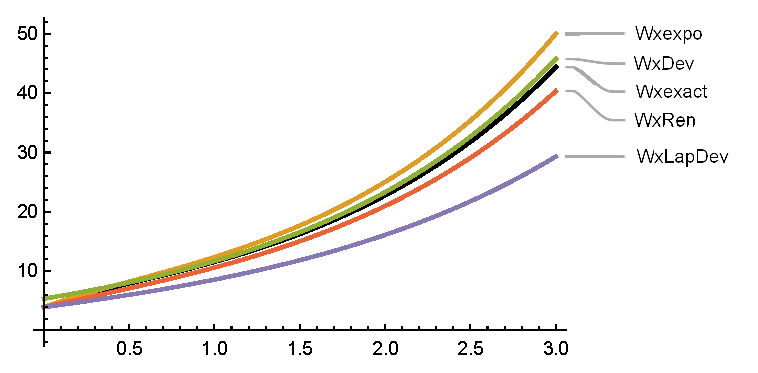
\includegraphics[width=\textwidth]{NH5mmW}
        \caption{$W_q(x)$ (in black)}
        \label{fig:NH5mmW}
    \end{subfigure}
    ~
    \\
    \begin{subfigure}[b]{0.8\textwidth}
        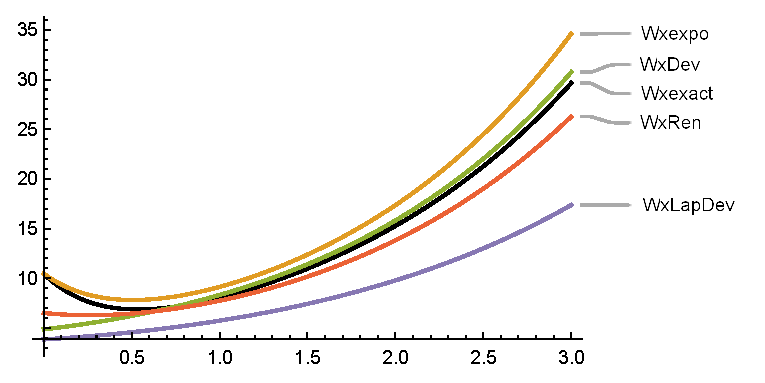
\includegraphics[width=\textwidth]{NH5mmW1}
        \caption{$W'_q(x) $}
        \label{fig:NH5mmW1}
    \end{subfigure}
    ~
    \\
    \begin{subfigure}[b]{0.8\textwidth}
        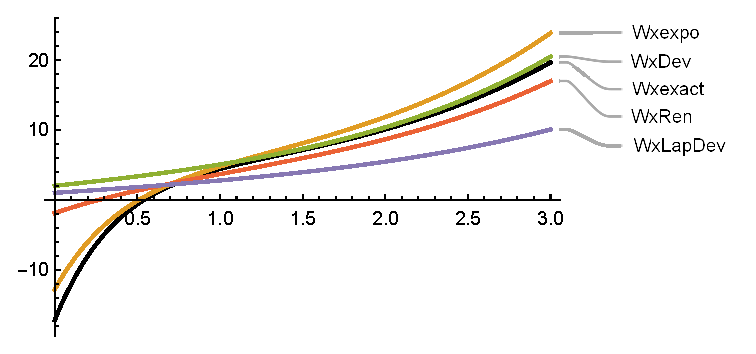
\includegraphics[width=\textwidth]{NH5mmW2}
        \caption{$W''_q(x)$}
        \label{fig:NH5mmW2}
    \end{subfigure}
    \caption{Plots of $W_q(x)$, $W'_q(x)$, and $W''_q(x)$ of the exact solution and the approximations, for $f(x)=\frac{5}{2 }e^{-5x}+\frac{4}{5} e^{-4 x}-\frac{1}{5}e^{-3x}- \frac{1}{5}e^{-2x}+ \frac{1}{20}e^{-x}$, $\theta=1$, $q=1/10$}
    \label{fig:NH5mm}
\end{figure}


As seen in table \ref{table:NH5mm}, the approximations for  $W_q$ give again the DeVylder as the closest approximation when looking at the $\Phi_q$ value. However, $W'_q$ for the DeVylder attains its minimum at $x=0$, which is relatively far from the exact barrier at $b_{DeF}=0.538$. The exponential approximation shows the best barrier approximate at $x=0.506947$.

The lack of a minimum of $W'_q$ for the DeVylder and the Laplace DeVylder approximations inside the interval $x \in (0,3)$ can be seen clearly in the plots in figure \ref{fig:NH5mmW1}. The lack of zero of the corresponding $W''_q$ plots in figure \ref{fig:NH5mmW2} supports this idea. The exponential approximation has the closest root to the exact at around $x=0.5$.

\begin{table}[!h]
\begin{tabular}{|l|l|l|l|l|}
\hline
       & \begin{tabular}[c]{@{}l@{}}Dominant   exponent \\ $\Phi_q$\end{tabular} & \begin{tabular}[c]{@{}l@{}}Percent   relative error\\ ($\Phi_q$)\end{tabular} & \begin{tabular}[c]{@{}l@{}}Optimal barrier\\ $b_{DeF}$\end{tabular} & \begin{tabular}[c]{@{}l@{}}Percent   relative error\\ ($b_{DeF}$)\end{tabular} \\ \hline
Exact  & 0.666084 & 0        & 0.538    & 0       \\ \hline
Expo   & 0.691616 & 3.8331   & 0.506947 & 5.77181 \\ \hline
Dev    & 0.670061 & 0.596931 & 0        & 100     \\ \hline
Renyi  & 0.650448 & 2.34749  & 0.260532 & 51.5739 \\ \hline
LapDev & 0.587976 & 11.7265  & 0        & 100     \\ \hline
\end{tabular}
\caption{Exact and approximate values of $\Phi_q$ and $b_{DeF}$ for $f(x)=\frac{5}{2 }e^{-5x}+\frac{4}{5} e^{-4 x}-\frac{1}{5}e^{-3x}- \frac{1}{5}e^{-2x}+ \frac{1}{20}e^{-x}$, $\theta=1$, $q=1/10$. The DeVylder approximation displayed the least percent relative error in approximating $\Phi_q$, but struggled in approximating $b_{DeF}$.}
\label{table:NH5mm}
\end{table}


\begin{table}[!h]
\begin{tabular}{|l|l|l|l|l|}
\hline
$\theta$ & Closest approximation & $\Phi_q$   exact & $\Phi_q$ approximation & \% error   $\Phi_q$ \\ \hline
1   & Dev                     & 0.666084       & 0.670061 & 0.596931          \\ \hline
0.9 & Dev                     & 0.721302       & 0.726797 & 0.761704          \\ \hline
0.8 & Dev                     & 0.785584       & 0.793322 & 0.985015          \\ \hline
0.7 & Dev                     & 0.861148       & 0.872279 & 1.29261           \\ \hline
0.6 & Dev                     & 0.950932       & 0.967325 & 1.72389           \\ \hline
0.5 & Dev                     & 1.05887        & 1.08366  & 2.34057           \\ \hline
0.4 & Dev                     & 1.19032        & 1.22891  & 3.24173           \\ \hline
0.3 & Dev                     & 1.35264        & 1.41474  & 4.59125           \\ \hline
0.2 & Dev                     & 1.55609        & 1.65988  & 6.6701            \\ \hline
0.1 & Expo                    & 1.81514        & 1.95652  & 7.78877           \\ \hline
\end{tabular}
\caption{Exact and approximate values of $\Phi_q$ for $f(x)=\frac{5}{2 }e^{-5x}+\frac{4}{5} e^{-4 x}-\frac{1}{5}e^{-3x}- \frac{1}{5}e^{-2x}+ \frac{1}{20}e^{-x}$, varying the value of $\theta$. The DeVylder approximation displayed the least percent relative error among the four approximations considered.}
\label{table:NH5mmPhiq}
\end{table}


\begin{table}[]
\begin{tabular}{|l|l|l|l|l|}
\hline
$\theta$ & Closest approximation & Barrier exact & Barrier approx & \% error Barrier \\ \hline
1   & Expo                    & 0.538           & 0.506947  & 5.77181            \\ \hline
0.9 & Expo                    & 0.496513        & 0.448391  & 9.69186            \\ \hline
0.8 & Expo                    & 0.448937        & 0.382485  & 14.8021            \\ \hline
0.7 & Expo                    & 0.394055        & 0.308318  & 21.7575            \\ \hline
0.6 & Expo                    & 0.330415        & 0.225085  & 31.8783            \\ \hline
0.5 & Expo                    & 0.256331        & 0.13227   & 48.3988            \\ \hline
0.4 & Expo                    & 0.169933        & 0.0299613 & 82.3687            \\ \hline
0.3 & Expo                    & 0.0693293       & 0         & 100                \\ \hline
0.2 & Exact                   & 0               & 0         & 0                  \\ \hline
0.1 & Exact                   & 0               & 0         & 0                  \\ \hline
\end{tabular}
\caption{Exact and approximate values of $\Phi_q$ for $f(x)=\frac{5}{2 }e^{-5x}+\frac{4}{5} e^{-4 x}-\frac{1}{5}e^{-3x}- \frac{1}{5}e^{-2x}+ \frac{1}{20}e^{-x}$, varying the value of $\theta$. The exponential approximation displayed the least percent relative error among the four approximations considered.}
\label{table:NH5mmBar}
\end{table} 